
% \begin{frame}{DOE ECP Acknowledgement}

% \textit{
% This research was supported by the Exascale Computing Project (17-SC-20-SC),
% a joint project of the U.S. Department of Energy’s Office of Science and National Nuclear Security Administration,
% responsible for delivering a capable exascale ecosystem, including software, applications, and hardware technology,
% to support the nation’s exascale computing imperative. 
% }

% \end{frame}

%==============================================================================
\ifnotoverview
\begin{frame}[fragile]

  \vspace{-10pt}

  {\Huge Introduction}

  \vspace{10pt}

  \textbf{Learning objectives:}
  \begin{itemize}
    \item{Why do we need Kokkos}
    \item{The Kokkos Ecosystem}
    \item{The Kokkos Team}
  \end{itemize}

  \vspace{-20pt}

\end{frame}
\fi

\begin{frame}[fragile]{The HPC Hardware Landscape}
  \begin{center}
    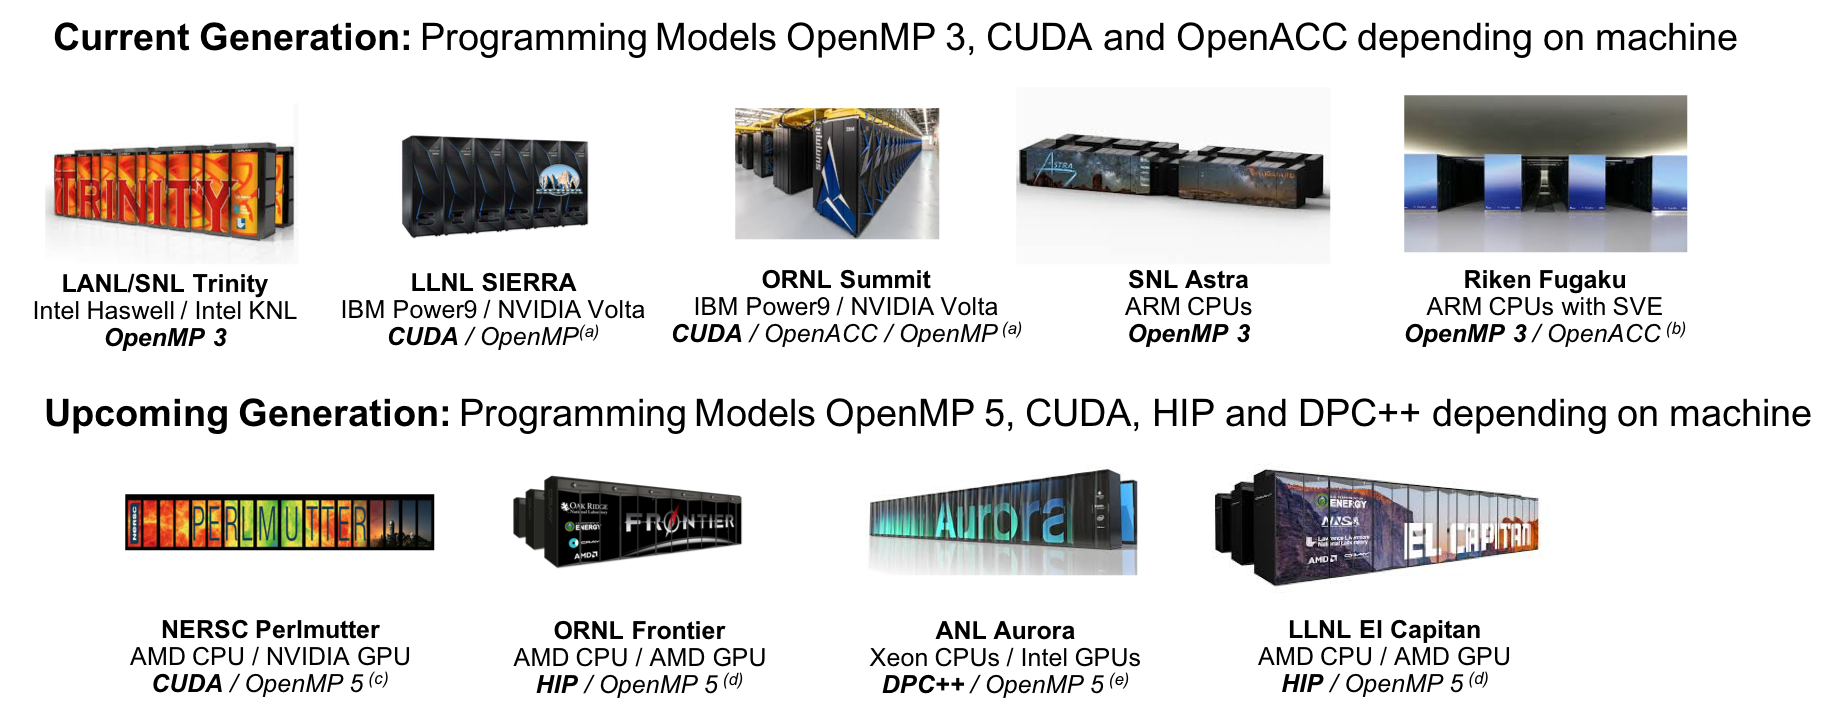
\includegraphics[width=1.05\textwidth]{figures/Architecture-Overview}
  \end{center}

  \begin{scriptsize}
  \emph{(a)} Initially not working. Now more robust for Fortran than C++, but getting better.

  \emph{(b)} Research effort.

  \emph{(c)} OpenMP 5 by NVIDIA.

  \emph{(d)} OpenMP 5 by HPE.

  \emph{(e)} OpenMP 5 by Intel.
  \end{scriptsize}

\end{frame}

\begin{frame}[fragile]{Cost of Coding}

\begin{block}{Industry Estimate}
A full time software engineer writes 10 lines of production code per hour: 20k LOC/year.
\end{block}

	\begin{itemize}
		\item Typical HPC production app: 300k-600k lines
			\begin{itemize}
				\item Sandia alone maintains a few dozen
			\end{itemize}
		\item Large Scientific Libraries:
			\begin{itemize}
				\item E3SM: 1,000k lines
				\item Trilinos: 4,000k lines
			\end{itemize}
	\end{itemize}

	\textbf{Conservative estimate:} need to rewrite 10\% of an app to switch Programming Model

	\pause

\begin{block}{Software Cost Switching Vendors}
Just switching Programming Models costs multiple person-years per app!
\end{block}

\end{frame}

\begin{frame}[fragile]{What is Kokkos?}
	\begin{itemize}
		\item A C++ Programming Model for Performance Portability
			\begin{itemize}
				\item Implemented as a template library on top CUDA, HIP, OpenMP, ...
				\item Aims to be descriptive not prescriptive
				\item Aligns with developments in the C++ standard
			\end{itemize}
		\item Expanding solution for common needs of modern science and engineering codes
			\begin{itemize}
				\item Math libraries based on Kokkos
				\item Tools for debugging, profiling and tuning
				\item Utilities for integration with Fortran and Python
			\end{itemize}
		\item It is an Open Source project with a growing community
			\begin{itemize}
				\item Maintained and developed at \url{https://github.com/kokkos}
				\item Hundreds of users at many large institutions
			\end{itemize}
	\end{itemize}
\end{frame}

\begin{frame}[fragile]{Kokkos at the Center}
  \begin{center}
    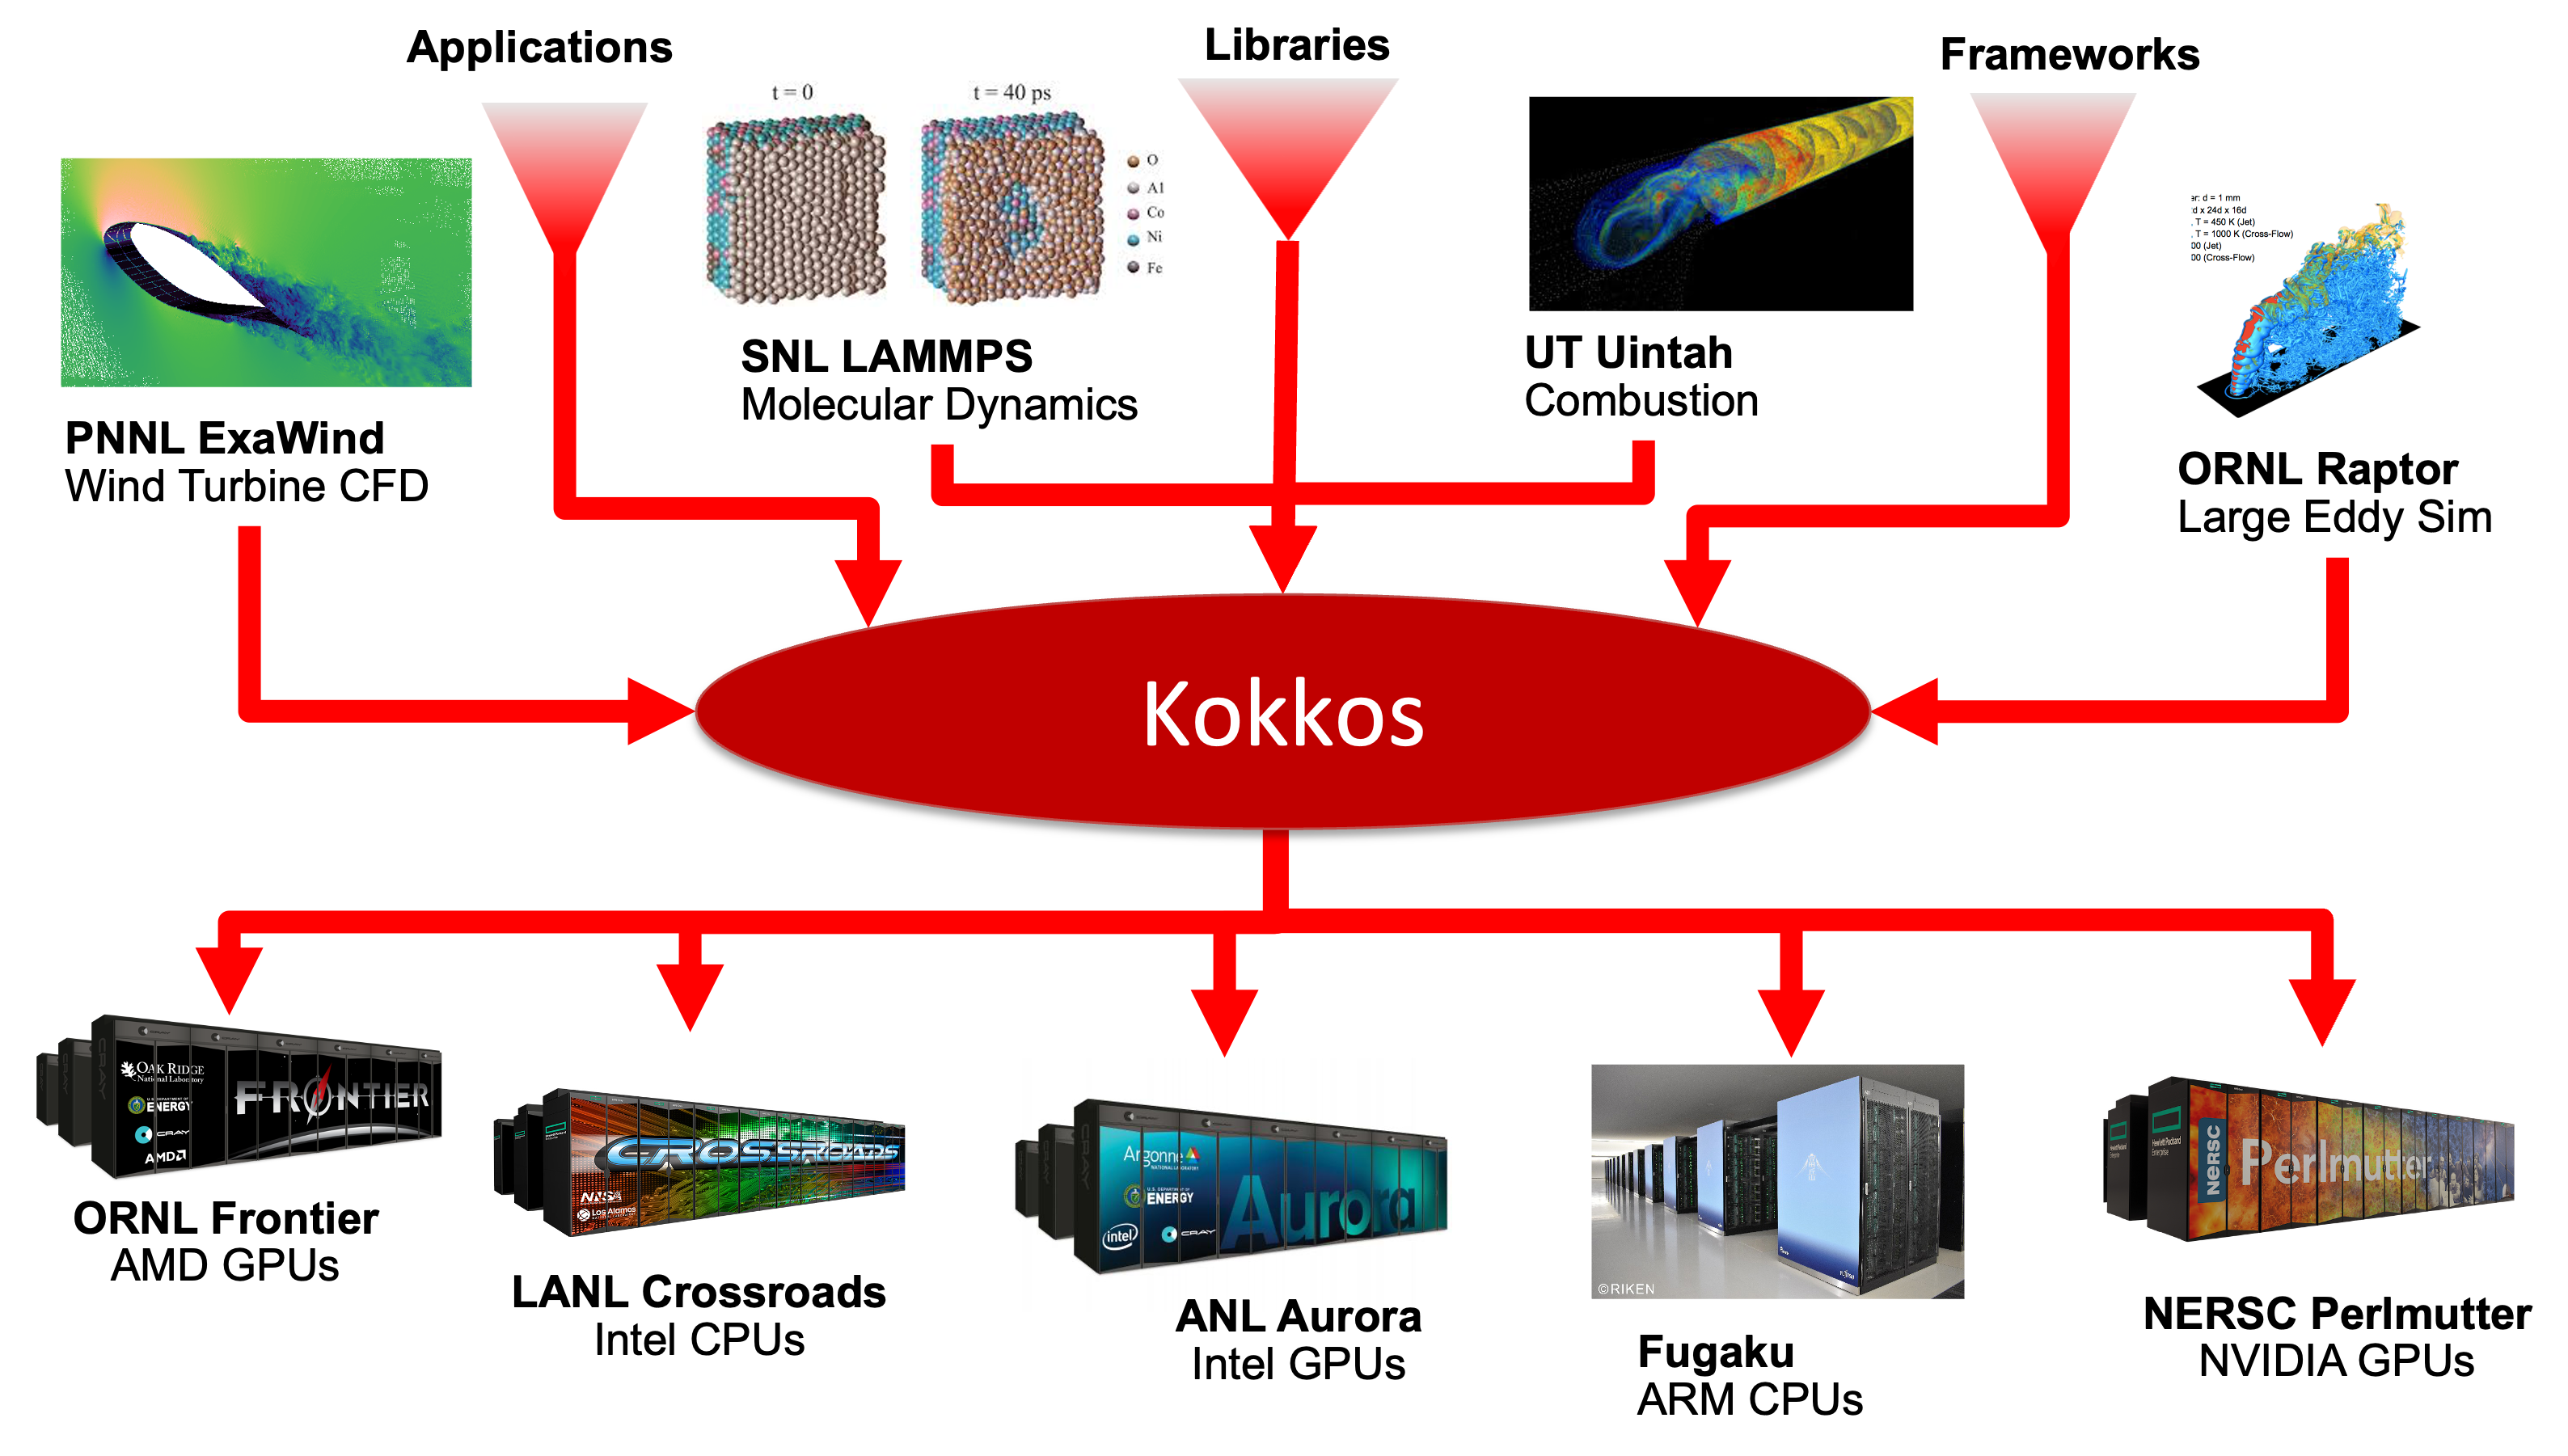
\includegraphics[width=1.05\textwidth]{figures/Kokkos-In-The-Middle-2024}
  \end{center}
\end{frame}

\begin{frame}[fragile]{The Kokkos Ecosystem}
  \begin{center}
    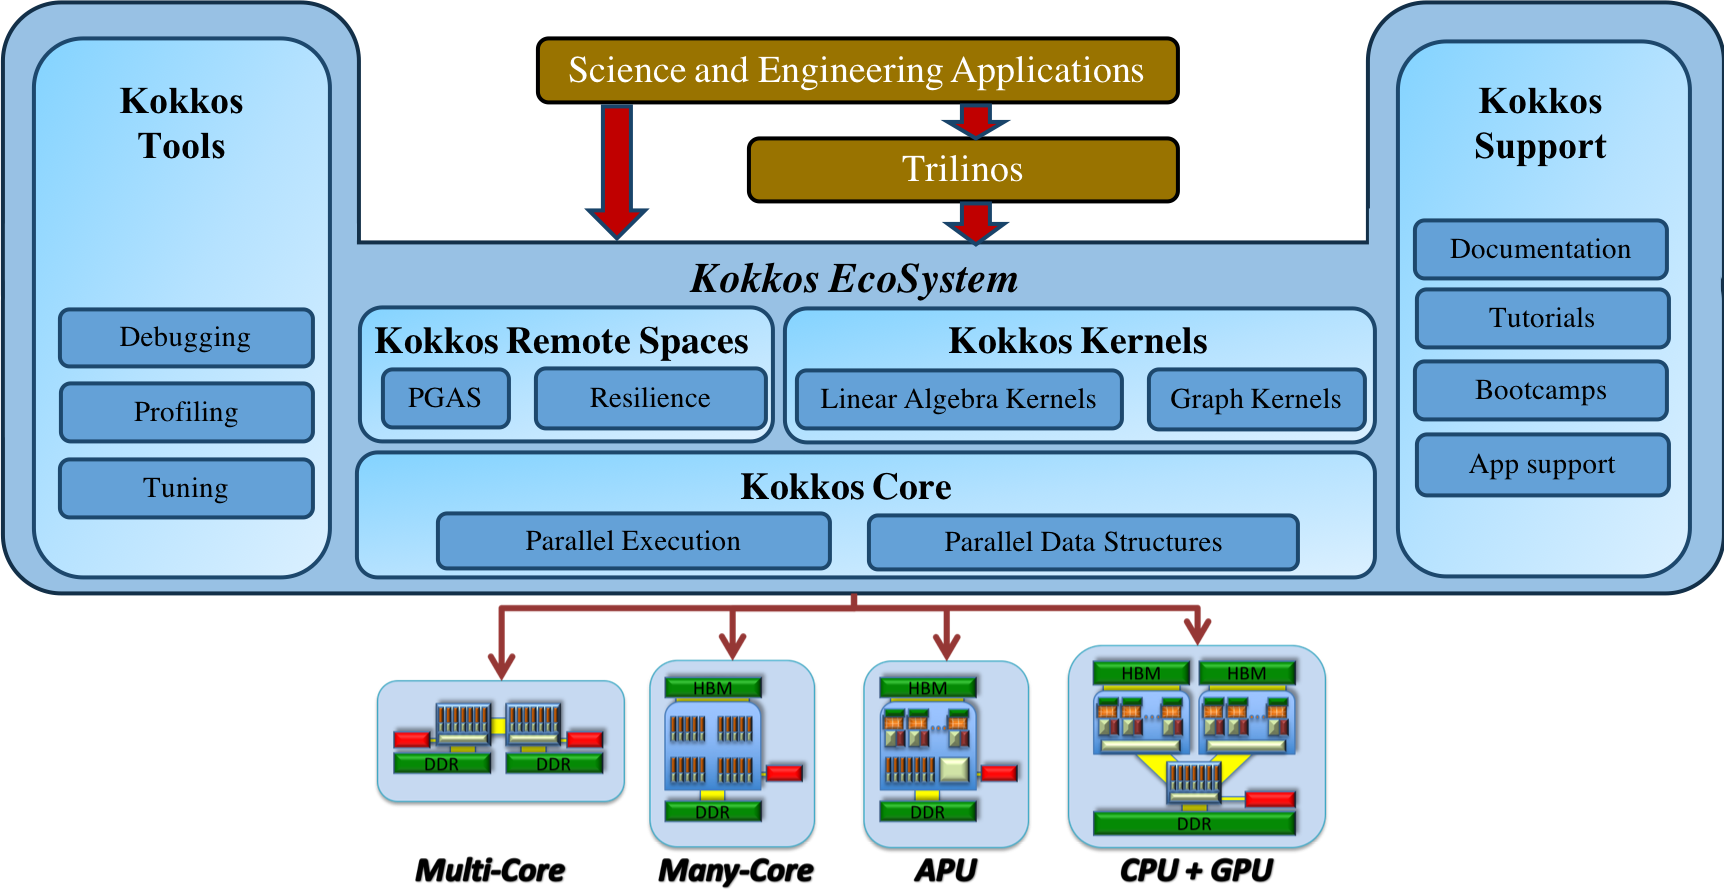
\includegraphics[width=1.05\textwidth]{figures/kokkos-eco-system}
  \end{center}
\end{frame}

\begin{frame}[fragile]{The Kokkos Team}
  \begin{center}
    
\includegraphics[width=0.9\textwidth]{figures/Kokkos-Team-2024}
  \end{center}
\end{frame}


\begin{frame}[fragile]{Kokkos and the C++ Standard}
  \textbf{Kokkos helps improve ISO C++}


	\vspace{-25pt}
\begin{center}                                                                                                                                    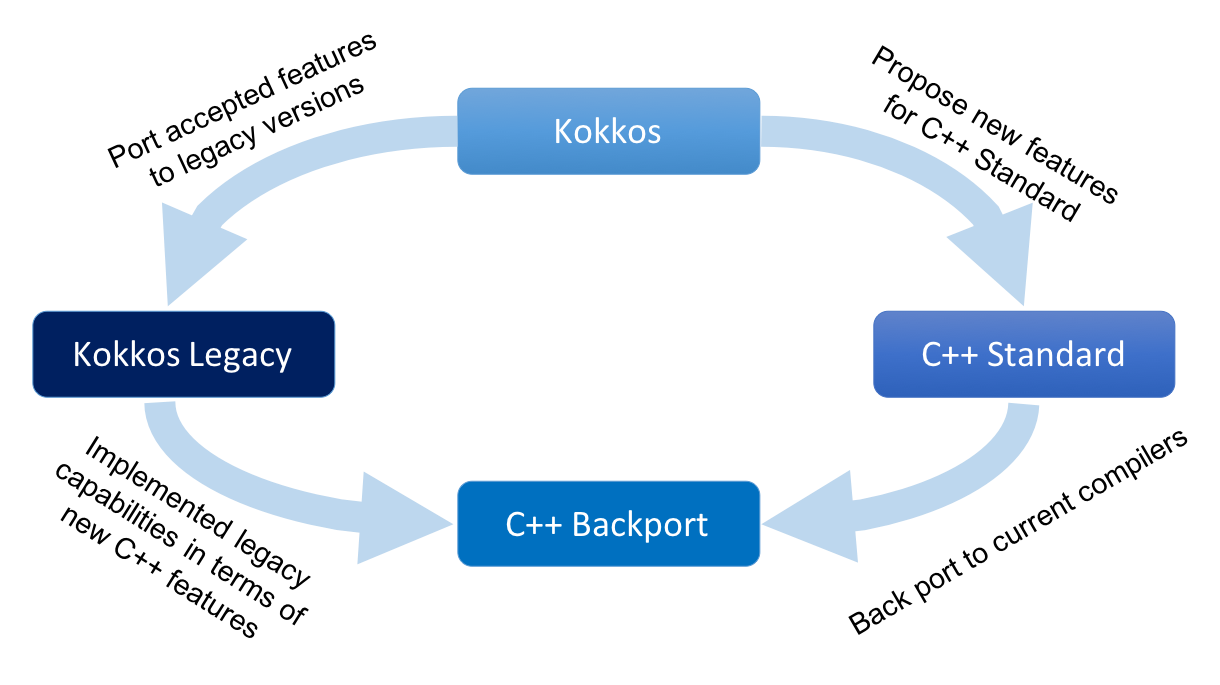
\includegraphics[width=1.05\textwidth]{figures/kokkos-cpp-standard}
\end{center}

	\vspace{-25pt}
\textit{Ten current or former Kokkos team members are members of the ISO C++ standard committee.}
\end{frame}

\iffull
\begin{frame}[fragile]{C++20 std::atomic\_ref}
	\textbf{C++11 std::atomic insufficient for HPC}
	\begin{itemize}
           \item Objects, not functions, with only atomic access
	   \item Can't use non-atomic access in one operation, and then atomic access in the next
	\end{itemize}

	\textbf{C++20 std::atomic\_ref adds atomic capabilites as in Kokkos}
	\begin{itemize}
		\item Can wrap standard allocations.
		\item Works also for sizes which can't be done lock-free (e.g. \texttt{complex$<$double$>$})
		\item Atomic operations on reasonably arbitrary types
	\end{itemize}

  \begin{code}[linebackgroundcolor={
      },
      keywords={atomic_add,atomic_ref}, frame=single
    ]
// Kokkos today
Kokkos::atomic_add(&a[i],5.0);

// atomic_ref in ISO C++20
std::atomic_ref(a[i]) += 5.0;
  \end{code}
\end{frame}
\fi

\iffull
\begin{frame}[fragile]{C++23 std::mdspan}
   \textbf{C++ does not provide multi dimensional arrays}
	\begin{itemize}
           \item Every scientific programming language has them: Fortran, Matlab, Python, ... 
	\end{itemize}

	\textbf{C++23 std::mdspan adds Kokkos::View like arrays}
	\begin{itemize}
		\item Reference semantics.
		\item Compile time and runtime extents (also mixed)
		\item Data layouts to allow for adapting hardware specific access patterns. 
		\item Subviews!
	\end{itemize}

  \begin{code}[linebackgroundcolor={
      },
      keywords={View,LayoutLeft,extents,mdspan,dynamic_extent,layout_left}, frame=single
    ]
// Kokkos today
View<float**[5],LayoutLeft> a("A",10,12); a(3,5,1) = 5;

// mdspan in ISO C++23
using ext = extents<int,dynamic_extent,dynamic_extent,5>;
mdspan<float,ext,layout_left> a(ptr,10,12); a[3,5,1]+=5;
  \end{code}

\end{frame}
\fi

\begin{frame}{Kokkos Users}
\textbf{Kokkos has a growing OpenSource Community}

\vspace{0.5cm}
\begin{itemize}
  \item 20 ECP projects list Kokkos as Critical Dependency
    \begin{itemize}
       \item 41 list C++ as critical
       \item 25 list Lapack as critical
       \item 21 list Fortran as critical
    \end{itemize}
  \item Slack Channel: 1.7k members from 100+ institutions
    \begin{itemize}
      \item 15\% Sandia Nat. Lab.
      \item 24\% other US Labs
      \item 22\% universities
      \item 39\% other
    \end{itemize}
  \item GitHub: 1.9k stars
\end{itemize}

\begin{tikzpicture}[remember picture,overlay]
    \node[xshift=-3.5cm,yshift=-6.5cm] at (current page.north east){%
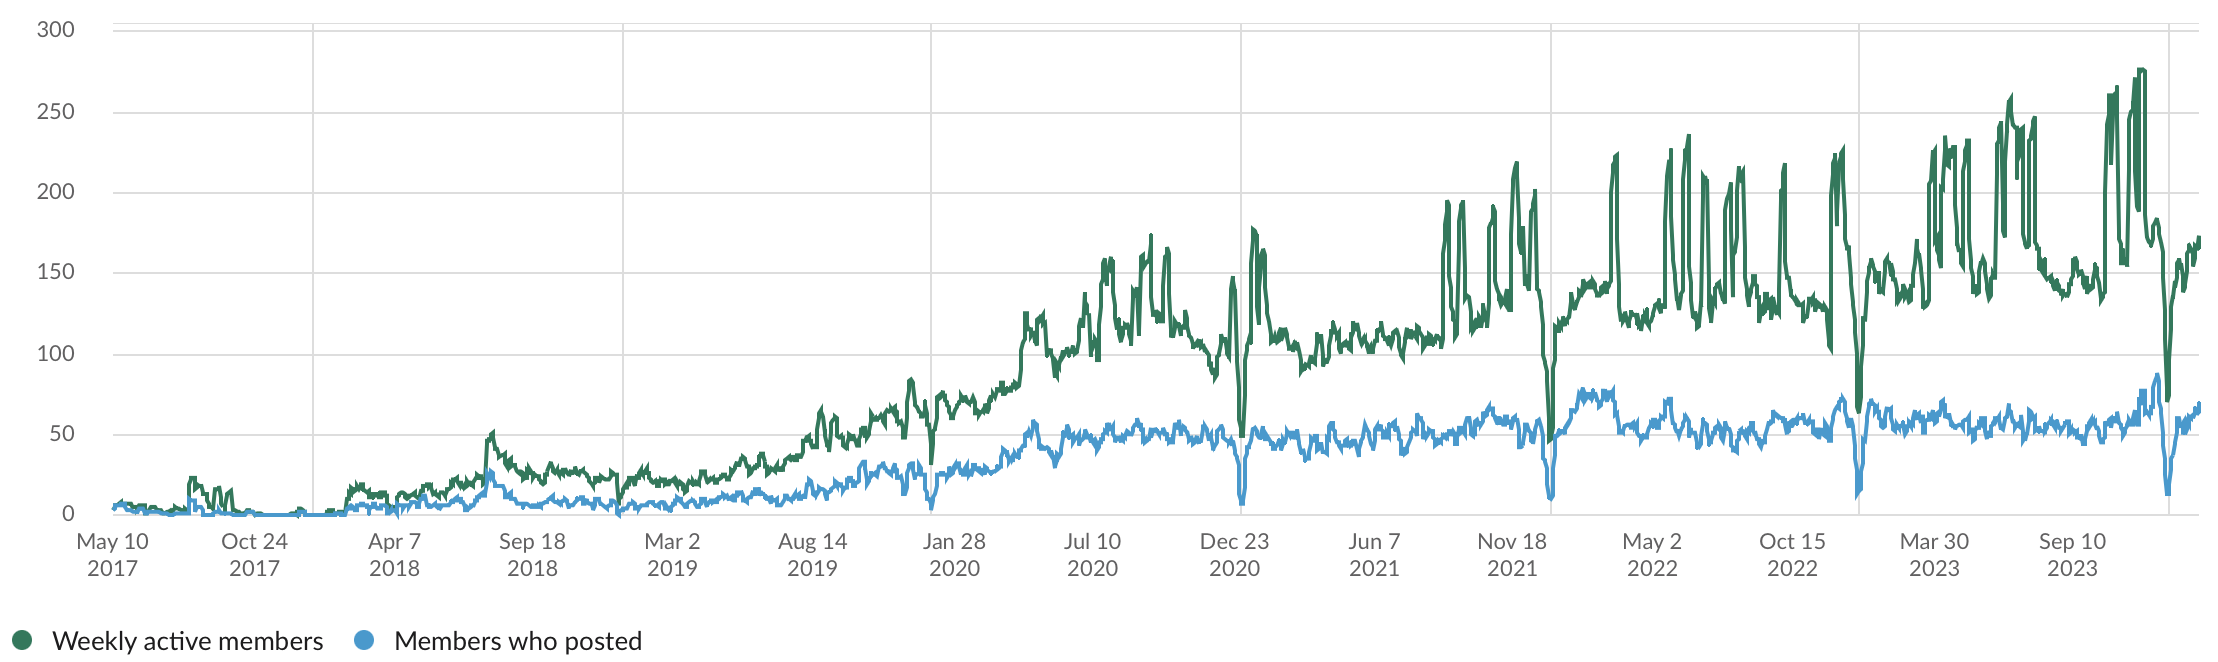
\includegraphics[width=6cm]{figures/KokkosSlack-Users-Feb24}
};
\end{tikzpicture}


\end{frame}
